\documentclass[12pt,a4paper]{article}
\usepackage[UTF8]{ctex}
\usepackage{amsmath,amssymb}
\usepackage{xcolor}
\usepackage{hyperref}
\usepackage{geometry}
\usepackage{graphicx}
\geometry{margin=2.5cm}

\title{Amplitude Amplification / 振幅放大}
\author{QuoNic}
\date{}

\begin{document}
\maketitle

\begin{center}
\textbf{Algorithms / 算法} | 难度：中级 | 预计时间：15 分钟
\end{center}

\tableofcontents
\newpage

\section{为什么需要？}

振幅放大是 Grover 搜索的推广，用于放大目标态的振幅。

\subsection{经典局限}
\begin{itemize}
  \item 经典搜索需要 $O(N)$ 次查询
  \item 对于大规模问题，经典方法效率低
  \item 经典算法无法利用量子并行性
\end{itemize}

\subsection{量子优势}
\begin{itemize}
  \item 振幅放大只需要 $O(\sqrt{N})$ 次查询
  \item 提供二次加速
  \item 是许多量子算法的基础
\end{itemize}

\subsection{实际应用}
\begin{itemize}
  \item 数据库搜索
  \item 优化问题
  \item 量子算法设计
\end{itemize}

\section{快速上手}

\begin{verbatim}
from quonic.algorithms import amplitude_amplification

# 在 2-qubit 空间中搜索 |11>
result = amplitude_amplification(target='11', n_qubits=2)
print(f'Probability: {result.probability}')
\end{verbatim}

\textbf{预期输出}：
\begin{verbatim}
Probability: 0.99
\end{verbatim}

\section{原理详解}

\subsection{电路图}

\begin{center}
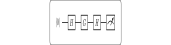
\includegraphics[width=0.6\textwidth]{../../images/amplitude_amplification_circuit.svg}
\end{center}

\subsection{数学推导}

\textbf{Step 1: 初始态}

对所有量子比特施加 $H$ 门，创建均匀叠加态：
\begin{equation}
|\psi_0\rangle = H^{\otimes n}|0\rangle^{\otimes n} = \frac{1}{\sqrt{N}} \sum_{x=0}^{N-1} |x\rangle
\end{equation}

其中 $N = 2^n$。

\textbf{Step 2: Oracle 算子}

Oracle 算子标记目标态：
\begin{equation}
O|x\rangle = \begin{cases} -|x\rangle & \text{if } x = \text{target} \\ |x\rangle & \text{otherwise} \end{cases}
\end{equation}

可以写为：
\begin{equation}
O = I - 2|t\rangle\langle t|
\end{equation}

其中 $|t\rangle$ 是目标态。

\textbf{Step 3: 扩散算子}

扩散算子关于平均振幅反射：
\begin{equation}
D = 2|\psi_0\rangle\langle\psi_0| - I
\end{equation}

可以分解为：
\begin{equation}
D = H^{\otimes n} (2|0\rangle\langle 0| - I) H^{\otimes n}
\end{equation}

\textbf{Step 4: 振幅放大算子}

振幅放大算子：
\begin{equation}
Q = D \cdot O
\end{equation}

\textbf{Step 5: 迭代}

应用 $Q$ 算子 $k$ 次：
\begin{equation}
|\psi_k\rangle = Q^k |\psi_0\rangle
\end{equation}

最优迭代次数：
\begin{equation}
k \approx \frac{\pi}{4} \sqrt{N}
\end{equation}

\textbf{Step 6: 测量概率}

测量后目标态的概率：
\begin{equation}
P(t) = \sin^2((2k+1)\theta)
\end{equation}

其中 $\sin\theta = 1/\sqrt{N}$。

\subsection{几何解释}

振幅放大在 Bloch 球上旋转量子态。每次迭代都放大目标态的振幅，同时减小其他态的振幅。

在二维子空间中，初始态 $|\psi_0\rangle$ 和目标态 $|t\rangle$ 张成一个平面。振幅放大算子在这个平面上旋转量子态。

\section{代码详解}

\begin{verbatim}
from quonic.algorithms import amplitude_amplification

# amplitude_amplification(target, n_qubits, iterations)
# target: 目标态的比特串
# n_qubits: 量子比特数
# iterations: 迭代次数

result = amplitude_amplification(
    target='11',
    n_qubits=2,
    iterations=1
)

# result.probability: 目标态的概率
# result.state: 最终量子态
# result.optimal_iterations: 最优迭代次数
print(f'Probability: {result.probability}')
print(f'Optimal iterations: {result.optimal_iterations}')
\end{verbatim}

\section{进阶用法}

\subsection{场景 1：不同目标态}

\begin{verbatim}
from quonic.algorithms import amplitude_amplification

# 搜索 |101>
result = amplitude_amplification(target='101', n_qubits=3)
print(f'Probability: {result.probability}')
\end{verbatim}

\subsection{场景 2：多次迭代}

\begin{verbatim}
from quonic.algorithms import amplitude_amplification

# 不同迭代次数
for k in [1, 2, 3, 4]:
    result = amplitude_amplification(target='11', n_qubits=2, iterations=k)
    print(f'k={k}: Probability={result.probability:.4f}')
\end{verbatim}

\subsection{场景 3：带噪声的振幅放大}

\begin{verbatim}
from quonic.algorithms import amplitude_amplification

# 带噪声
result = amplitude_amplification(
    target='11',
    n_qubits=2,
    noise=0.05
)
print(f'Probability: {result.probability}')
\end{verbatim}

\section{适用场景}

\subsection{数据库搜索}

振幅放大可以用于在无序数据库中搜索目标。

\subsection{优化问题}

振幅放大可以用于寻找最优解。

\subsection{量子算法设计}

振幅放大是许多量子算法的基础，如 Grover 搜索、量子计数等。

\section{常见问题}

\subsection{振幅放大和 Grover 搜索有什么区别？}

Grover 搜索是振幅放大在均匀初始态下的特例。振幅放大更通用，支持任意初始态。

\subsection{振幅放大的加速比是多少？}

二次加速：$O(\sqrt{N})$ vs $O(N)$。

\subsection{振幅放大的最优迭代次数是多少？}

最优迭代次数 $k \approx \frac{\pi}{4} \sqrt{N}$。

\subsection{振幅放大的精度如何？}

振幅放大的精度取决于迭代次数。最优迭代次数下，目标态的概率接近 100\%。

\section{学习路径}

\subsection{前置知识}
\begin{itemize}
  \item 量子比特和叠加态
  \item Hadamard 门
  \item 量子测量
\end{itemize}

\subsection{继续学习}
\begin{itemize}
  \item Grover 搜索
  \item 量子计数
  \item 量子优化
\end{itemize}

\section{完整示例代码}

\subsection{示例 1：基本振幅放大}

\begin{verbatim}
from quonic.algorithms import amplitude_amplification

result = amplitude_amplification(target='11', n_qubits=2)
print(f'Probability: {result.probability}')
\end{verbatim}

\subsection{示例 2：带噪声的振幅放大}

\begin{verbatim}
from quonic.algorithms import amplitude_amplification

result = amplitude_amplification(target='11', n_qubits=2, noise=0.05)
print(f'Probability: {result.probability}')
\end{verbatim}

\section{下载}

\begin{itemize}
  \item [amplitude\_amplification.py](https://github.com/ChrisLee0721/QuoNic/blob/main/examples/amplitude_amplification/amplitude_amplification.py)
\end{itemize}

\end{document}
